\documentclass[]{article}
\usepackage[T1]{fontenc}
\usepackage{lmodern}
\usepackage{amssymb,amsmath}
\usepackage{fullpage}
\usepackage{ifxetex,ifluatex}
\usepackage{fixltx2e} % provides \textsubscript
% use microtype if available
\IfFileExists{microtype.sty}{\usepackage{microtype}}{}
\ifnum 0\ifxetex 1\fi\ifluatex 1\fi=0 % if pdftex
  \usepackage[utf8]{inputenc}
\else % if luatex or xelatex
  \usepackage{fontspec}
  \ifxetex
    \usepackage{xltxtra,xunicode}
  \fi
  \defaultfontfeatures{Mapping=tex-text,Scale=MatchLowercase}
  \newcommand{\euro}{€}
\fi
% Redefine labelwidth for lists; otherwise, the enumerate package will cause
% markers to extend beyond the left margin.
\makeatletter\AtBeginDocument{%
  \renewcommand{\@listi}
    {\setlength{\labelwidth}{4em}}
}\makeatother
\usepackage{enumerate}
\usepackage{graphicx}
% We will generate all images so they have a width \maxwidth. This means
% that they will get their normal width if they fit onto the page, but
% are scaled down if they would overflow the margins.
\makeatletter
\def\maxwidth{\ifdim\Gin@nat@width>\linewidth\linewidth
\else\Gin@nat@width\fi}
\makeatother
\let\Oldincludegraphics\includegraphics
\renewcommand{\includegraphics}[1]{\Oldincludegraphics[width=\maxwidth]{#1}}
\ifxetex
  \usepackage[setpagesize=false, % page size defined by xetex
              unicode=false, % unicode breaks when used with xetex
              xetex]{hyperref}
\else
  \usepackage[unicode=true]{hyperref}
\fi
\hypersetup{breaklinks=true,
            bookmarks=true,
            pdfauthor={Harshal Pandya and Brian Martin},
            pdftitle={CS677: Lab 1},
            colorlinks=true,
            urlcolor=blue,
            linkcolor=magenta,
            pdfborder={0 0 0}}
\setlength{\parindent}{0pt}
\setlength{\parskip}{6pt plus 2pt minus 1pt}
\setlength{\emergencystretch}{3em}  % prevent overfull lines
\setcounter{secnumdepth}{0}

\title{CS677: Lab 2}
\author{Brian Martin and Harshal Pandya}
\date{}

\begin{document}
\maketitle

Our system implements the provided spec: a pig2pig network in which pigs
collaborate to avoid impact with an adversarial bird. The pigs dynamically 
elect a leader amongst themselves and use Lamport's clocks for synchronization.

\subsection{Actors}
We use the Actor framework to enable communication between machines. The
Actor model is a mathematical model of concurrent computation that
treats ``actors'' as the universal primitives of concurrent digital
computation: in response to a message that it receives, an actor can
make local decisions, create more actors, send more messages, and
determine how to respond to the next message received. Each actor is multi-threaded 
and can send/receive messages concurrently. Moreover, we can specify whether we want 
synchronous or asynchronous semantics.

\subsection{Leader Election}
We use the ring based leader election algorithm to enable the pigs to choose a leader dynamically.
Each pig gets a random 8-digit Id at start up and the pigs organize in a logical ring in an arbitrary order.
The network topology is completely connected which allows the pigs to reorganize into a new ring in the
event one of the nodes fails. Any pig can start the election. A message is circulated along the ring and every 
pig attaches its Id to the message and passes it on. When the initiator receives the message it, it picks the 
pig with the highest Id that is alive, informs everyone about the new leader. We use a timeout to figure whether 
a pig is down and move on if the pig does not respond within a particular interval.

\subsection{Clock Synchronization}
We use Lamport's clocks to order events across the pigs. When the leader initiates the game by sending the BirdApproaching 
message it sends along its current time to all pigs. The pigs use this value to update their clocks setting it to the max of remote 
and local clock. We simulate the network latency by incrementing the clock randomly (to a value up to 5) before processing the
bird approaching message. If the pig is able to move, the clock is advanced and the time is stored as Move Time. \\
After the time to target as specified by the bird has expired the leader sends a BirdLanded message to all pigs again with its time stamp. 
The pigs simulate the network delay and after comparing the time stamp, save it as Hit Time.\\
When the leader queries the pigs for their status, they respond by comparing these clock values to decide if they were able to move before the bird hit. 
Obviously, all this happens only if the pig is impacted by the bird's landing.  

\subsection{Game Map}

The game map is single-dimensional with pigs and columns placed
randomly. It is assumed that the bird is always launched from the left
(as in the original Angry Birds). The ratio of columns to pigs is at
most one.

\subsection{Assumed Physics}

We assume that certain behaviors for each element type:

\begin{itemize}
\item
  \textbf{Pig}: An impacted pig will fall to the right (as the bird
  always approaches from the left). If a pig falls onto another pig both
  are considered impacted, but the second pig does not change position
  on impact. If a pig is impacted while having a column to the right,
  then that column will also fall to the right, affecting any pig which
  may find itself in that position.
\item
  \textbf{Column}: If a column is impacted directly, then it falls to
  the right, only affecting any pig or column to its immediate right.
\end{itemize}

\subsection{Game Engine}

In our system the \emph{game engine} has several roles:

\begin{enumerate}[1.]
\item
  Map generation
\item
  Sending round-initiating trajectory message to the leader.
\item
  Querying the leader for the status of pigs. 
\end{enumerate}

\subsection{Pigs as Actors}

Each pig functions as an actor which can receive and act on several
message types, derived from the original specification. Some of them are listed below,
please refer to the doc provided for exhaustive list.

\begin{itemize}
\item
  \texttt{Trajectory(position: Int,timeToLive: Int)} notifies the leader about the
  birds trajectory.
\item
  \texttt{BirdApproaching(targetPosition: Int, timestamp: LamportClock)} used by
  the leader to initiate a round of notifications the pig being
  hit.
\item
  \texttt{Status()} used to query each pig about its safety.
\item
  \texttt{Election()} to start an election.
\end{itemize}

\subsection{Launching a bird}

A bird launch is described by the time the master picks a random target
and notifies the nearest pig about the trajectory. It then picks a
random time to target before sending an end game message thus signaling
that the bird has landed.

\section{Design Decisions / Trade-offs}

The pigs form a completely connected netowork topology and so hopcounts are 
not required. However, this increases the complexity of the network and it may not scale well 
for larger number of nodes.The pigs don't maintain any state apart from their current
locations in the world.\\
We choose ring based election algorithm since it involves no synchronization issues and
is fairly robust to failures. However we make a simplifying assumption that a pig never goes down 
within a round. If this was not the case we would need to back up the state of the leader and have 
it communicate to each pig after every event so that it is up to date with the state of every pig.\\
Lamport's clocks are convenient for this problem since they have much less 
overhead than vector clocks. Since we are only comparing local timestamps and
the messages from the leader are broadcast, we can prove the correctness of the ordering.\\
We do not maintain a shared map data structure and hence the map is not
updated when the pigs move. This however saves the effort of maintaing a
synchronous thread-safe data structure that lives on the master and adds
extra messages to the system.

\section{Possible Improvements}

We could experiment with allowing the pigs to fail while a round is being played. 
In terms of the game logic, we could use a 2
dimensional world. Also we could make pigs move make space for pigs
being affected and have the effect of hits cascade beyond 2 positions.

\section{How to run the program}

We require \texttt{maven}, the Java dependency management tool, to pull
in all dependencies and generate a jar file of compiled code.

We have included two scripts in the code directory:

\begin{enumerate}[1.]
\item
  \textbf{\texttt{bin/install.sh}}: This will retrieve all the
  dependencies, compile the source.
\item
  \textbf{\texttt{bin/run.sh}}: This will run several rounds of the
  game, running through all of the test cases (shown on the following
  page).
\end{enumerate}

\pagebreak

\section{Test cases:}

%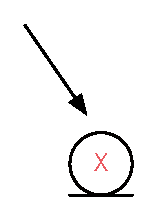
\includegraphics{figs/test1.pdf} 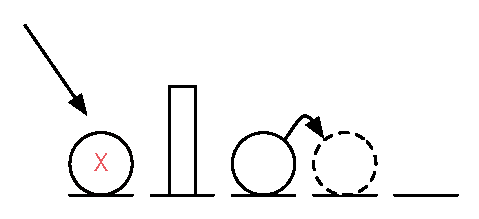
\includegraphics{figs/test2.pdf}
%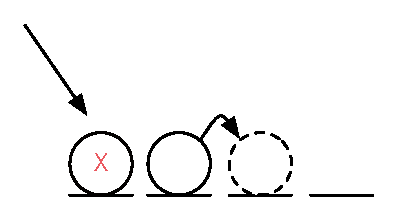
\includegraphics{figs/test3.pdf} 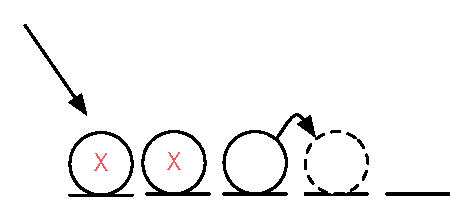
\includegraphics{figs/test4.pdf}
%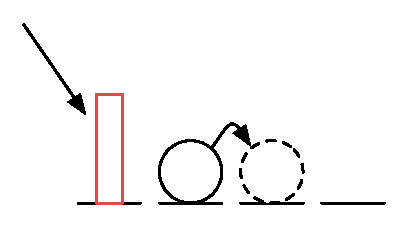
\includegraphics{figs/test5.pdf}

\section{Sample Output:}

When running the pigs:

\begin{verbatim}
Starting pig on port: 10001
Starting pig on port: 10002
Starting pig on port: 10003
Starting pig on port: 10004
Starting pig on port: 10005
Starting pig on port: 10006
Starting pig on port: 10007
Starting pig on port: 10008
Starting pig on port: 10009
Starting pig on port: 10010
\end{verbatim}

When running the game:

\begin{verbatim}
Gathering Pigs...
Looking up on port: 10001
Checking alive: Position(-1)
Looking up on port: 10002
Checking alive: Position(-1)
Looking up on port: 10003
Checking alive: Position(-1)
Looking up on port: 10004
Checking alive: Position(-1)
Looking up on port: 10005
Checking alive: Position(-1)
Looking up on port: 10006
Checking alive: Position(-1)
Looking up on port: 10007
Checking alive: Position(-1)
Looking up on port: 10008
Checking alive: Position(-1)
Looking up on port: 10009
Checking alive: Position(-1)
Looking up on port: 10010
Checking alive: Position(-1)
done gathering.
Can we communicate with the first pig?: Position(-1)
done setting mid positions
done setting end positions

  -----------------------
  |  Initial locations  |
  -----------------------

       |                 |     |                 |        | 
 @  _  |  _  _  @  @  @  |  @  |  @  _  @  @  @  |  @  _  | 
------------------------------------------------------------
Time to target: 589

  -----------------------
  |  Final locations    |
  -----------------------


       |                 |     |                 |        | 
 @  _  |  _  _  @  @  @  |  @  |  @  _  @  @  @  |  @  _  | 
------------------------------------------------------------
                           XXX                                    <- TARGET
\end{verbatim}

\end{document}
